\documentclass{article}
\usepackage[utf8]{inputenc}
\usepackage[T1]{fontenc}
\usepackage{graphicx}
\usepackage{hyperref}
\usepackage{geometry}
\geometry{margin=1in}

\title{CABENIA}
\date{Encyclopaedia Britannica (1771)}

\begin{document}
\maketitle

\section*{Historical source}
\textbf{Entry ID:} \texttt{entry-cabenia-2464} \\
\textbf{Volume ID:} 144133902 \\
\textbf{Character Count:} 98

\subsection*{Extracted Text}
CABENIA, a pre-town of Congo, in Africa, and fubied to the Portuguese: E. Long-129, and B. lat. 4.



\section*{Source record}
\begin{itemize}
\item \textbf{Dataset:} \texttt{NationalLibraryOfScotland/encyclopaedia\_britannica\_illustrated}
\item \textbf{Dataset Revision:} \texttt{309f765b1ecc83e0a7f7762e44b4a927a7555443}
\item \textbf{Page ID:} \texttt{britannica:309f765b1ecc83e0a7f7762e44b4a927a7555443:train:2464} \\
  \textbf{Filename:} \texttt{page-2464-24f450326eee.jpg} \\
  \textbf{Row Index:} 2464 \\
  \textbf{SHA256:} \texttt{24f450326eee13b0...}
\end{itemize}

\begin{figure}[h]
\centering
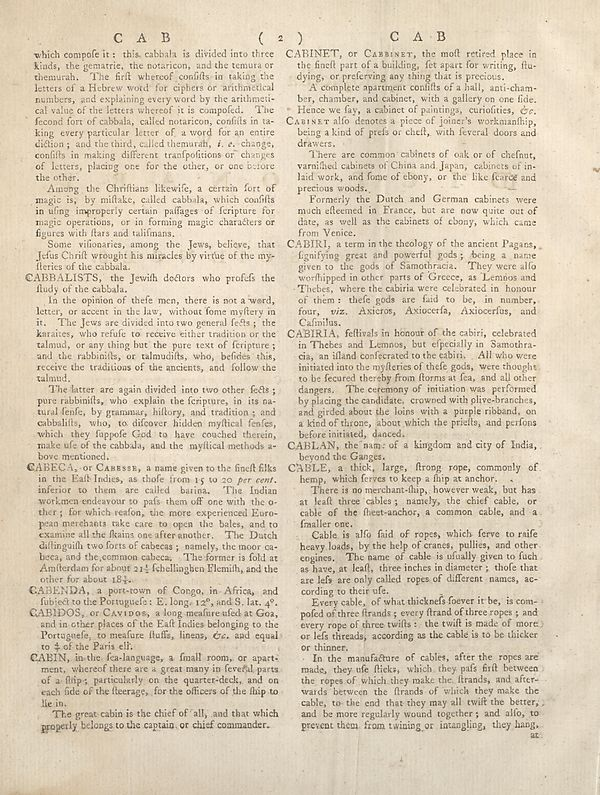
\includegraphics[width=0.85\textwidth]{../scans/page-2464-24f450326eee.jpg}
\caption*{Source scan: \texttt{page-2464-24f450326eee.jpg}}
\end{figure}

\end{document}
